\chapter{Ergänzungen zur Laufzeitanalyse von Parsivald}
\label{appendix_runtime}

\section{Einfluss der Ereignis-Laufzeit auf die effiziente Raumgröße\texorpdfstring{$w_\text{eff}$}{weff}}

Die Ereignis-Laufzeit $T_\text{E}$ hat einen ähnlichen Einfluss auf $w_\text{eff}$ wie die MD-Laufzeit $T_\text{MD}$, doch ergibt sich eine inverse Proportionalität $w_\text{eff} \sim T_\text{E}^{-1}$, wie in Abbildung~\ref{fig:weffeventtime} zu erkennen ist.
Dieser Zusammenhang ergibt sich aus dem höheren Ereignisdurchsatz $R_\text{E}$ des Hauptprozesses, mit dem $p_\text{max,2}$ steigt.
Somit verschiebt sich die Grenze $w_\text{eff}$, für die $p_\text{max,1} = p_\text{max,2}$ gilt, weiter nach oben, wodurch größere Räume effizient betrachtet werden können.

\begin{figure}[p]

  \captionsetup[subfigure]{singlelinecheck=false}
  \def\subfigwidth{7cm}
  \begin{subfigure}[t]{\subfigwidth}
    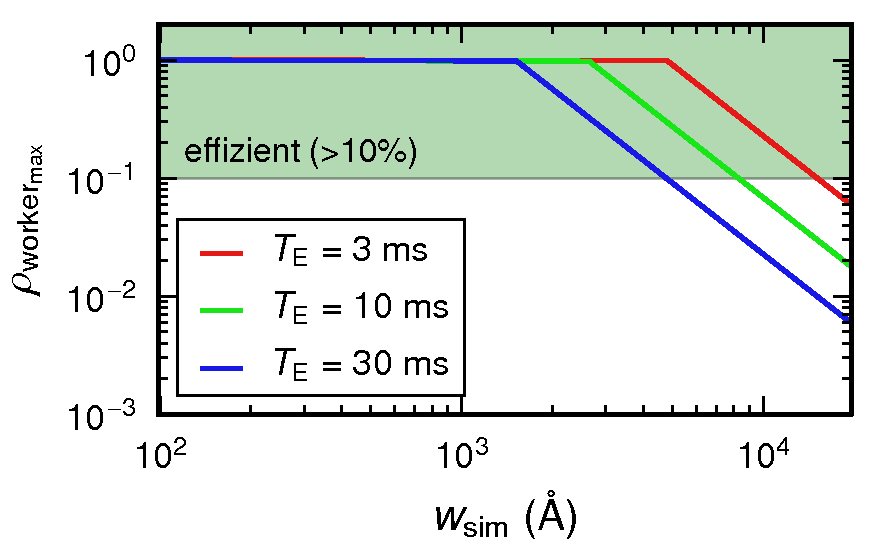
\includegraphics[width=\textwidth]{densitybykmctime}
  \end{subfigure}
  \hfill
  \begin{subfigure}[t]{\subfigwidth}
    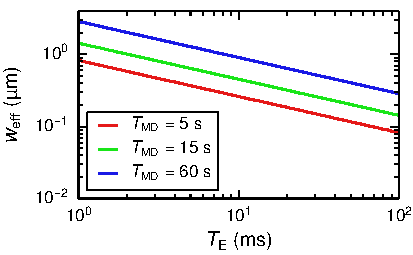
\includegraphics[width=\textwidth]{maxsizebykmctime}
  \end{subfigure}

  \caption{Einfluss der Ereignis-Laufzeit $T_\text{E}$ auf die effiziente Simulationsgröße $w_\text{eff}$}
  \label{fig:weffeventtime}

\end{figure}

\section{Zusätzliche Einflüsse auf das Maximum der Prozesse \texorpdfstring{$p_\text{max}$}{pmax}}

Zusätzlich zur Ereignis- und MD-Laufzeit wird $p_\text{max}$ über die Größe der MD-Boxen $w_\text{MD}$ und die maximale Workerdichte $\rho_\text{worker,max}$ während der Simulation beeinflusst (Abbildung~\ref{fig:pmaxother}).
$\rho_\text{worker}$ ist dabei von der Verteilung der Adsorptionsorte auf der Oberfläche abhängig und hat für gleichverteilte Simulationen von Gold-PVD Werte zwischen \SI{10}{\percent} und \SI{20}{\percent} angenommen.
Für stärker lokalisierte Adsorptionen sind aufgrund der überlappenden MD-Boxen und der daraus resultierenden Abhängigkeit der Ereignisse geringere Werte für $\rho_\text{worker}$ zu erwarten.
Es gilt $w_\text{eff} \sim \rho_\text{worker,max}^{-1}$

Die Erhöhung von $w_\text{MD}$ hat umfangreichere Einflüsse und verursacht eine Verringerung von $\rho_\text{max}$ aufgrund der Größe der Box, sowie eine Erhöhung von $T_\text{MD}$ und $T_\text{E}$ aufgrund der größeren Zahl an Atomen in der Box, was insgesamt zu einer Erhöhung von $w_\text{eff}$ führt.
Somit wird $p_\text{max}$ für $w_\text{sim} < w_\text{eff}$ verringert und für $w_\text{sim} > w_\text{eff}$ erhöht.
Da mit der Vergrößerung der MD-Boxen auch die gesamte Laufzeit nahezu proportional skaliert (Abbildung~\ref{fig:tpother}), wird $w_\text{MD}$ meistens minimal gewählt.

\begin{figure}[p]

  \captionsetup[subfigure]{singlelinecheck=false}
  \def\subfigwidth{7cm}
  \begin{subfigure}[t]{\subfigwidth}
    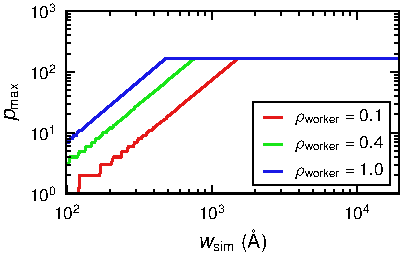
\includegraphics[width=\textwidth]{workersbydensity}
  \end{subfigure}
  \hfill
  \begin{subfigure}[t]{\subfigwidth}
    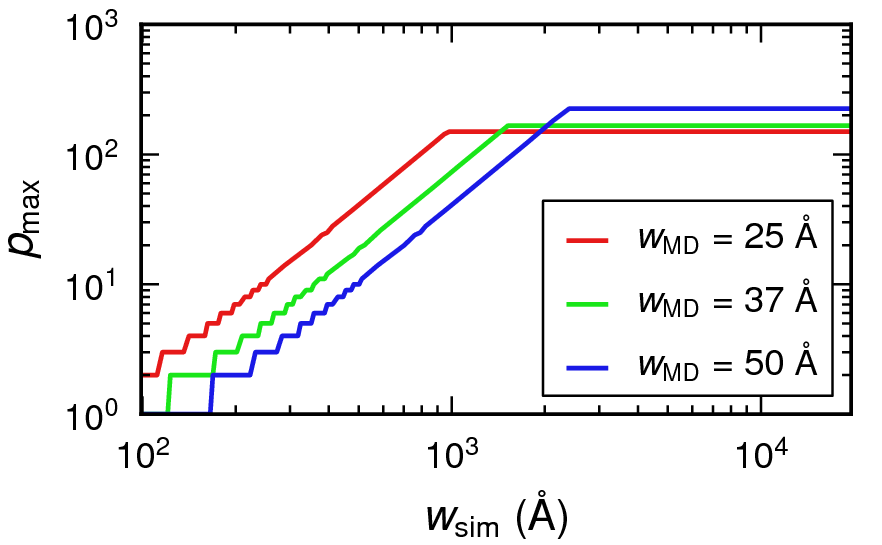
\includegraphics[width=\textwidth]{workersbymdsize}
  \end{subfigure}

  \caption{Einfluss von $\rho_\text{worker}$ und $w_\text{MD}$ auf das Maximum von Prozessen $p_\text{max}$}
  \label{fig:pmaxother}

\end{figure}

\begin{figure}[p]

  \captionsetup[subfigure]{singlelinecheck=false}
  \def\subfigwidth{7cm}
  \begin{subfigure}[t]{\subfigwidth}
    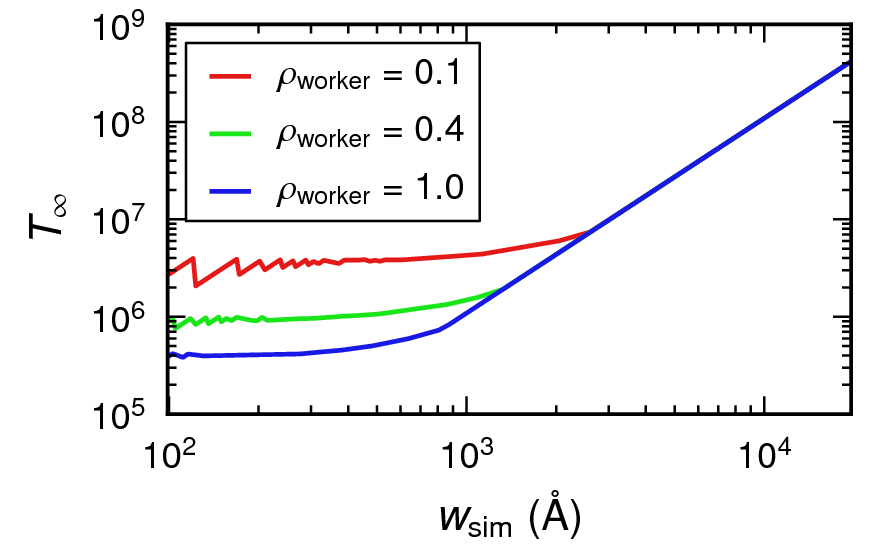
\includegraphics[width=\textwidth]{runtimebydensity}
  \end{subfigure}
  \hfill
  \begin{subfigure}[t]{\subfigwidth}
    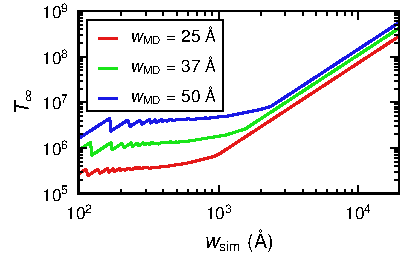
\includegraphics[width=\textwidth]{runtimebymdsize}
  \end{subfigure}

  \caption{Einfluss von $\rho_\text{worker}$ und $w_\text{MD}$ auf die Laufzeit $T_p$}
  \label{fig:tpother}

\end{figure}

\clearpage

\section{Abschätzung der maximalen Workerdichte per Random Sequential Adsorption}
\label{appendix_rsamaxdensity}

Bei Random Sequential Adsorption (RSA) werden geometrische Objekte nichtüberlappend an zufälligen Positionen in einem Raum verteilt, bis kein weiteres Objekt platziert werden kann.
Die Verteilung der quadratischen Worker auf der Oberfläche geschieht auf eine ähnliche Weise, sodass als Grenzwert der Workerdichte \SI{56.2}{\percent}\cite{brosilow_random_1991} angegeben werden kann.

Da Parsivald die Ereignisorte mit KMC-Methoden wählt, muss die zeitliche Reihenfolge der Ereignisse eingehalten werden, weshalb die überdeckenden Ereignisse nicht verworfen werden, sondern bis zum Abschluss des überdeckten Ereignisses zurück gestellt werden und sich so ein kompletter Abhängigkeitsbaum aufbaut, wie er in meiner Bachelorarbeit wird\cite{lorenz_entwicklung_2012}.
Dadurch kollidieren die MD-Boxen zurückgestellter Ereignisse mit nachfolgenden Ereignissen, welche wiederum zurückgestellt werden müssen.
Somit reduziert sich das Maximum der Workerdichte für große Simulationsräume auf den Grenzwert von \SI{25.95}{\percent} (Abbildung~\ref{fig:rsamaxdensity}).
Dieser Wert wurde über eine modifizierte RSA-Simulation ermittelt, die auf diese Parsivald-Methode der Ereignisauswahl und -Durchführung angepasst wurde.

KMC-Ereignisse werden in Parsivald für geringe Zeiträume durch einen trivialen Warte\-schlangen-Algorithmus vorausberechnet, um eine hohe Parallelisierbarkeit zu ermöglichen.
Um häufige Revisionen der Ereignisse und damit verbundene Leistungseinbußen zu vermeiden, wird die Tiefe der Abhängigkeitsbäume der Ereignisse beschränkt, was sich in einer verminderten Zahl von Versuchen zur Erzeugung eines neuen KMC-Ereignisses äußert.
Im Gegenzug sinkt damit die Workerdichte auf die für Gold-PVD und Kupfer-PVD in den Abschnitten~\ref{goldpvd} und~\ref{copperpvd} beobachteten Werte von \SIrange{10}{20}{\percent}.

\vspace{2em}

\begin{figure}[h]
  \centering
  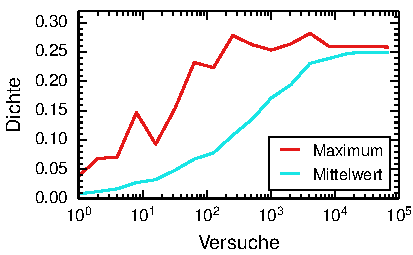
\includegraphics[width=10cm]{rsa_maxdensity}

  \caption[Abschätzung der maximalen Workerdichte per RSA-Simulation]{
    Abschätzung der maximalen Workerdichte durch eine modifizierte RSA-Simulation.
    Als Grenzwert für viele KMC-Versuche ergibt sich \SI{25.95}{\percent}
  }
  \label{fig:rsamaxdensity}

\end{figure}
